\capitulo{6}{Estado del arte}

En este apartado se va a aportar una visión más amplia del \quotes{estado del arte} mediante el estudio de otras herramientas similares.

\section{Weka-STPM}
WEKA for Moving Object Data Analysis and Mining o Weka-STPM es una extensión para Weka que permite soportar de forma automática el procesado de trayectorias o rutas para añadir semántica a las mismas. Está desarrollada por la Doctora Vania Bogorny, profesora del Departamento de Informática y Estadística en la Universidad Federal de Santa Catarina (Brasil).

Inicialmente parece una herramienta clave que podía haber facilitado el análisis de las rutas puesto que permitía la lectura y escritura en Bases de Datos PostgreSQL y soportaba la extensión PostGIS, pero tras algunas pruebas se vio que no se obtenían los resultados esperados.

Además, se puede ver por su código, que no está completamente terminada, encontrándose algunos errores en su ejecución y opciones no disponibles. Por ejemplo, aunque se lograba una conexión contra la Base de Datos, no se lograba que la aplicación insertase ningún tipo de resultado en la misma.

Su interfaz (Figura \ref{weka}) basada en Swing tampoco ayuda a comprender su funcionamiento puesto que hay botonoes que quedan ocultos, opciones que no se visualizan y desplegables que desaparecen detrás del resto de menús. Ante los problemas encontrados no se puede afirmar que esta herramienta pueda ser de gran utilidad en la actualidad pero sí es posible garantizar que si su desarrollo finaliza supondrá un gran paso adelante en el análisis de cualquier tipo de trayectoria.

\begin{figure}[h]
  \centering
    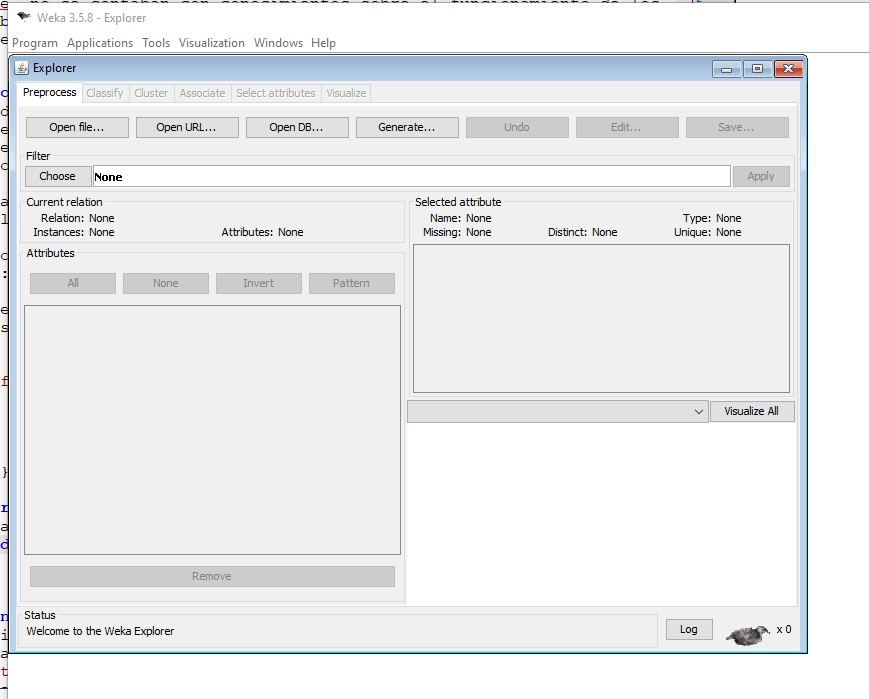
\includegraphics[width=0.6\textwidth]{../img/weka/weka.jpg}
  \caption{Interfaz sencilla de weka.}
  \label{weka}
\end{figure}


\section{CARTO}
Carto es una plataforma de cómputo en la nube SaaS (Software as a Service) que provee de un sistema de información geográfica o GIS y herramientas de mapeo de información para navegadores web.

Está basada en la extensión PostGIS de ProstreSQL y es de código abierto. Su \textit{front-end} está basado en JavaScript mientas que su \textit{back-end} está basado en Node.js.

El aspecto que muestran los mapas creados mediante CARTO puede ser visto en la Figura \ref{carto}.

\begin{figure}[h]
  \centering
    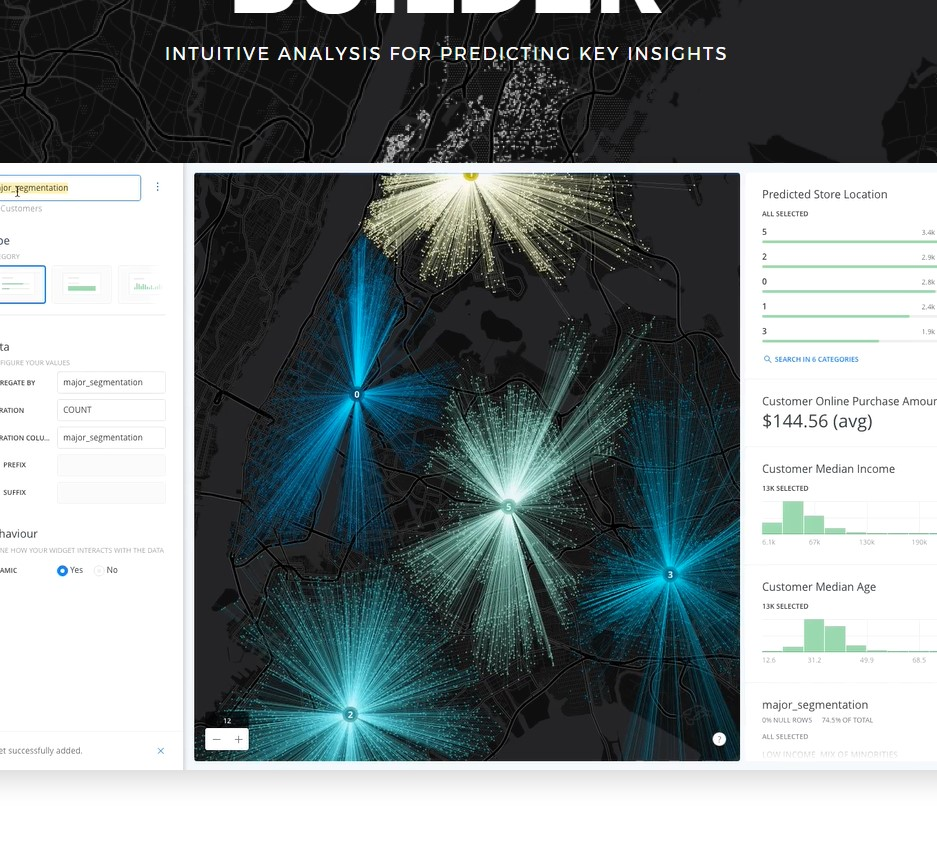
\includegraphics[width=0.6\textwidth]{../img/weka/carto.jpg}
  \caption{Aspecto final de los mapas en CARTO.}
  \label{carto}
\end{figure}


\subsection{CARTO Builder}
CARTO Builder es una aplicación web en la que los usuarios pueden procesar sus datos, realizar anaálisis y diseñar mapas propios. CARTO Builder está pensado y diseñado para todas las personas noveles que desean hacer uso de estas herramientas sin contar con conocimientos previos ni avanzados en sistemas de información geográficos. No obstante se provee de acceso a consultas SQL que pueden ser personalizadas si se cuenta con mayores conocimientos.

\subsection{CARTO Engine}
CARTO Engine provee al usuario de distintas APIs y librerías que permiten la construcción de mapas completamente personalizados.

\begin{itemize}
	\item SQL: se pueden hacer uso de todas las sentencias SQL soportadas en PostgreSQL.
	\item Mapas: permite obtener distintas plantillas de mapas en base a los requerimientos del usuario. De esta forma, cada usuario puede diseñar un mapa propio que usar en una aplicación web.
	\item Servicio de datos: permite desarrollar una mayor funcionalidad como el \textbf{geocoding}.
\end{itemize}

Aunque como se puede apreciar, su gran variedad de características permite una amplia capacidad de análisis de datos pudiendo ser una herramienta potente y de interesante uso, no se adapta al completo a los requerimientos iniciales de este proyecto, por lo que se decidió no hacer uso de la misma.

\section{Google Trips}

Quizá la primera aproximación a esta aplicación pueda parecer que es la que más se adapta al espíritu de este proyecto. Google Trips (Figura \ref{trips}) permite organizar viajes o rutas en pocos minutos.

También facilita obtener sugerencias de sitios no visitados que guardan relación con los visitados anteriormente y que hayan gustado a su usuario, preparar rutas diarias, organizar reservas según un calendario en Gmail, etc.

\begin{figure}[h]
  \centering
    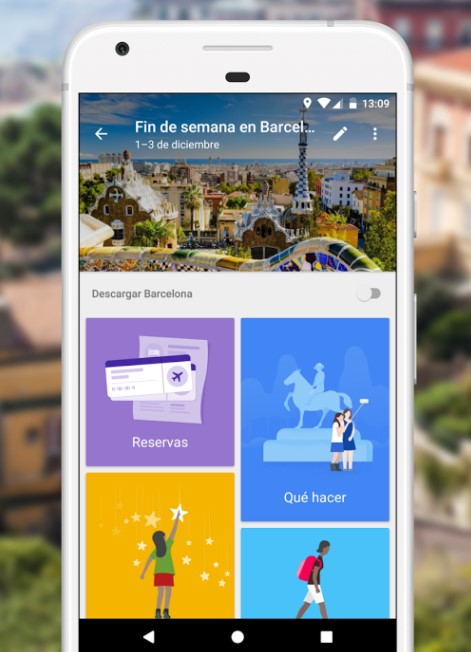
\includegraphics[width=0.6\textwidth]{../img/weka/trips.jpg}
  \caption{Aspecto de la interfaz de la aplicación Google Trips.}
  \label{trips}
\end{figure}

Pero el aspecto que esta aplicación móvil no realiza es el análisis y asignación de semántica a rutas ya realizadas, aspecto que diferencia la plataforma desarrollada con esta aplicación.


\section{Conclusiones sobre el estado del arte}

Como se ha visto en los apartados anteriores, existe una variedad interesante de plataformas y/o aplicaciones desarrolladas con el afán del análisis y/o gestión de rutas basadas en coordenadas GPS. Si bien existen más plataformas similares a las mencionadas, en esta sección se han mostrado las juzgadas como más interesantes.

Comparando sus características se puede ver que estas plataformas no permiten asignar semántica a trayectorias basadas en coordenadas geográficas. Por tanto, se puede afirmar que por los ejemplos mostrados en esta sección de la documentación, la aplicación web aquí mostrada añade nuevas funcionalidades a los sistemas existentes.

Por último, cabe destacar que, la plataforma desarrollada está completamente basada en tecnologías y datos libres de los que cualquier usuario puede hacer uso.


